%-------------------------------------------------------------------------------
% seq64_midi_formats
%-------------------------------------------------------------------------------
%
% \file        seq64_midi_formats.tex
% \library     Documents
% \author      Chris Ahlstrom
% \date        2015-09-03
% \update      2018-10-31
% \version     $Revision$
% \license     $XPC_GPL_LICENSE$
%
%     Provides a discussion of the formats (legacy and new) of the last
%     track of an Seq24/Sequencer64 MIDI file.
%
%-------------------------------------------------------------------------------

\section{MIDI Format and Other MIDI Notes}
\label{sec:midi_format_and_midi_notes}

\subsection{Standard MIDI Format 0}
\label{subsec:midi_format_smf_0}

   \index{smf 0}
   \index{channel split}
   \textsl{Sequencer64} can read and import SMF 0 MIDI files, and performs
   channel splitting automatically.
   When an SMF 0 format is detected, \textsl{Sequencer64}
%  reads the file as if were an SMF 1 file, but
   puts all of the events into the
   same sequence/pattern.  While the file is being processed, a list of the
   channels present in the track is maintained.

   Tempo and Time Signature events are read, if present.
   When saving a \textsl{Sequencer64} MIDI file,
%  in non-legacy mode,
   the Tempo and Time Signature events are saved as MIDI events.
   \index{new!time/tempo saved}
   This allows other sequencers to read a \textsl{Sequencer64} MIDI file.
   This addition of Tempo can fix imported tracks that don't have a
   measure value.
%  (e.g. it has 0 instead of at least one measure) associated
%  with them; unfixed, these tracks have racing progress bars that don't
%  reflect the actually progresss through the track.

   Once the end-of-track is encountered for that pattern, one new empty
   pattern is created for each channel found in the original sequence.
   The events in the main patten are scanned, one by one, and added at the
   end of the appropriate patten.  If the event is a channel event,
   then the event is inserted into the patten that was created for that
   channel.  If the event is a non-channel event, then each patten gets a
   copy of that event.

   After processing, the MIDI buss information, track name, and other pieces of
   information are attached to each sequence.  The following figure shows in
   imported SMF 0 tune, split into tracks.

\begin{figure}[H]
   \centering 
   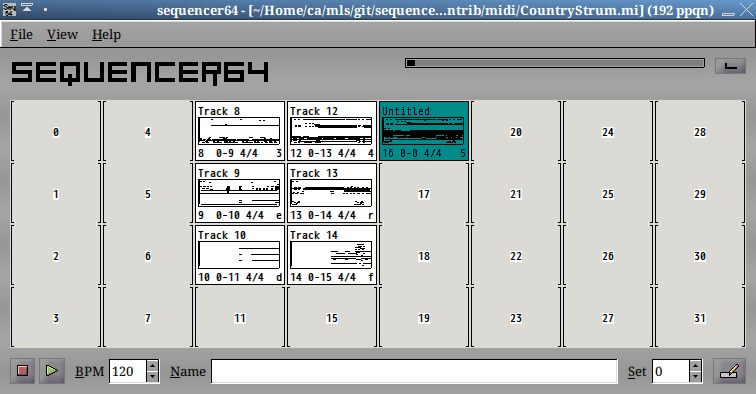
\includegraphics[scale=0.65]{smf0/imported-smf-0-song.png}
   \caption{Imported SMF 0 MIDI Song}
   \label{fig:imported_smf_0_song}
\end{figure}

   The imported SMF 0 track is preserved, in
   pattern slot \#16.  It is highlighted in a dark cyan color to remind the
   user that it is a special \textsl{Sequencer64} pattern.
%  It has no channel number.  It is
%  assigned the non-existent MIDI channel of 0.
   If the original track had no
   title, this track is named "Untitled".
   One will either delete
   this track before saving the file, or keep it muted.

   Each single-channel track is given a title of either the form
   "N: Track-name" or, if the song was untitled, "Track N".
   The sequence number of each new track is the internal channel number
   (always the actual MIDI channel number minus one).
   The time-signature of each track is set to defaults, unless a
   time-signature event is encountered in the imported file.

   \index{tempo events}
   \index{time signature events}
   \textsl{Sequencer64} supports reading some other
   information a MIDI SMF 0 track might have, such as the Tempo and the
   Time Signature.  It saves this information in the first track
   of the MIDI file.
   The original SMF 0 track is also shown in the song editor, as in the
   following figure.

\begin{figure}[H]
   \centering 
   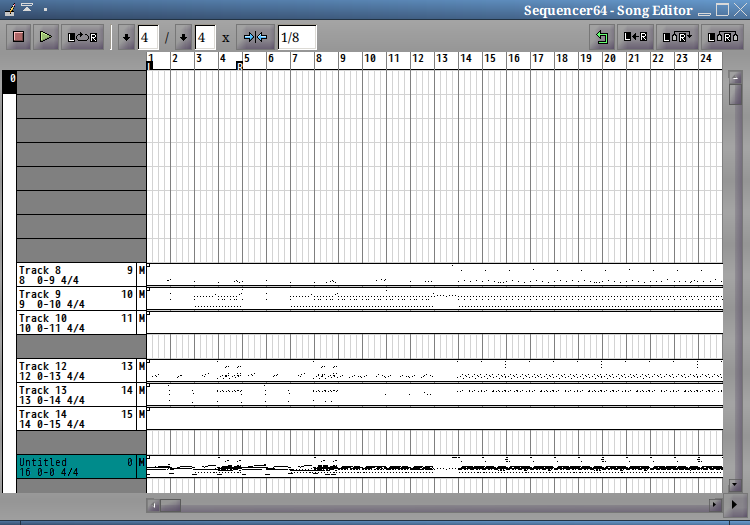
\includegraphics[scale=0.65]{smf0/imported-smf-0-song-editor.png}
   \caption{SMF 0 MIDI Song in the Song Editor}
   \label{fig:imported_smf_0_song_editor}
\end{figure}

   One is free to edit the imported tune to heart's content.
   Here, we added one instance of each track, including the SMF 0 track,
   to show what the imported song looks like.

\subsection{Legacy Proprietary Track Format}
\label{subsec:legacy_midi_format}

   The authors of \textsl{Seq24} took trouble to ensure that the format
   of the MIDI files it writes are compatible with other MIDI applications.
   \textsl{Seq24} also stores its own information (triggers, MIDI control
   information, etc) in the file, but marked so that other sequencers can read
   the file and ignore its \textsl{Seq24}-specific information.

   \textsl{Sequencer64} continues that MIDI-compliant behavior, but has
   improved the compliance a bit. 
   We call that last chunk of sequencer-specific information the "proprietary
   track".
   Before we discuss that last, proprietary track, note that the normal MIDI
   tracks that
   precede it include the SeqSpec ("sequencer-specific")
   control tags.
%  shown in \tableref{table:seqspec_items_normal_tracks}.
%  These control tags are global constants in the \textsl{Seq24} source
%  code, ranging from 0x24240001 to 0x24240013.
%
%  \begin{table}[htb]
%     \centering
%     \caption{SeqSpec Items in Normal Tracks}
%     \label{table:seqspec_items_normal_tracks}
%     \begin{tabular}{l l}
%        \texttt{c\_midibus}        & \texttt{24 24 00 01 00 00 00 00} \\
%        \texttt{c\_midich}         & \texttt{24 24 00 02 00 00 00 00} \\
%        \texttt{c\_triggers}       & \texttt{24 24 00 04 00 00 00 00} \\
%        \texttt{c\_timesig}        & \texttt{24 24 00 06 00 00 00 00} \\
%        \texttt{c\_triggers\_new}  & \texttt{24 24 00 08 00 00 00 00} \\
%        \texttt{c\_musickey}       & \texttt{24 24 00 11 00} \\
%        \texttt{c\_musicscale}     & \texttt{24 24 00 12 00} \\
%        \texttt{c\_backsequence}   & \texttt{24 24 00 13 00 00 00 00} \\
%     \end{tabular}
%  \end{table}
%

   All of the SeqSpecs are shown in the next table.
   The \texttt{c\_triggers} tag is obsolete, but still present.

   \begin{table}[htb]
      \centering
      \caption{All SeqSpec Items}
      \label{table:seqspec_items_all}
      \begin{tabular}{l l}
         \texttt{c\_midibus}        & \texttt{24 24 00 01 00 00 00 00} \\
         \texttt{c\_midich}         & \texttt{24 24 00 02 00 00 00 00} \\
         \texttt{c\_midiclocks}     & \texttt{24 24 00 03 00 00 00 00} \\
         \texttt{c\_triggers}       & \texttt{24 24 00 04 00 00 00 00} \\
         \texttt{c\_notes}          & \texttt{24 24 00 05 00 00 00 00} \\
         \texttt{c\_timesig}        & \texttt{24 24 00 06 00 00 00 00} \\
         \texttt{c\_bpmtag}         & \texttt{24 24 00 07 00 00 00 00} \\
         \texttt{c\_triggers\_new}  & \texttt{24 24 00 08 00 00 00 00} \\
         \texttt{c\_mutegroups}     & \texttt{24 24 00 09 00 00 00 00} \\
         \texttt{c\_gap\_A}         & \texttt{24 24 00 0A 00 00 00 00} \\
         \texttt{c\_gap\_B}         & \texttt{24 24 00 0B 00 00 00 00} \\
         \texttt{c\_gap\_C}         & \texttt{24 24 00 0C 00 00 00 00} \\
         \texttt{c\_gap\_D}         & \texttt{24 24 00 0D 00 00 00 00} \\
         \texttt{c\_gap\_E}         & \texttt{24 24 00 0E 00 00 00 00} \\
         \texttt{c\_gap\_F}         & \texttt{24 24 00 0F 00 00 00 00} \\
         \texttt{c\_midictrl}       & \texttt{24 24 00 10 00} \\
         \texttt{c\_musickey}       & \texttt{24 24 00 11 00} \\
         \texttt{c\_musicscale}     & \texttt{24 24 00 12 00} \\
         \texttt{c\_backsequence}   & \texttt{24 24 00 13 00 00 00 00} \\
         \texttt{c\_transpose}      & \texttt{24 24 00 14 00 00 00 00} \\
         \texttt{c\_perf\_bp\_mess} & \texttt{24 24 00 15 00 00 00 00} \\
         \texttt{c\_perf\_bw}       & \texttt{24 24 00 16 00 00 00 00} \\
         \texttt{c\_tempo\_map}     & \texttt{24 24 00 17 00 00 00 00} \\
         \texttt{c\_reserver\_1}    & \texttt{24 24 00 18 00 00 00 00} \\
         \texttt{c\_reserver\_2}    & \texttt{24 24 00 19 00 00 00 00} \\
         \texttt{c\_tempo\_track}   & \texttt{24 24 00 1A 00 00 00 00} \\
         \texttt{c\_seq\_color}     & \texttt{24 24 00 1B 00 00 00 00} \\
         \texttt{c\_seq\_edit\_mode} & \texttt{24 24 00 1C 00 00 00 00} \\
      \end{tabular}
   \end{table}

   \index{saved control tags}
   The \texttt{c\_musickey},
   \texttt{c\_musicscale}, and
   \texttt{c\_backsequence}
   control tags are new with \textsl{Sequencer64}.
   They are saved as additional information in each sequence in which they
   have been specified in the sequence editor.
   For backward compatibility (and because it is probably the more
   common use case), these items can also be
   saved globally for the whole MIDI song, as an option.

   These tags
%  (created by the application, but not present in the
%  proprietary track, and perhaps also created by other MIDI applications)
   are preceded by the standard MIDI "FF 7F length" meta-event sequence.
   The following discussion applies to the final "proprietary" track as
   saved in the legacy \textsl{Seq24} format.

   After all the counted MIDI event
   tracks are read, \textsl{Seq24} checks for
   extra data after them.
   If there is extra data, \textsl{Seq24} reads a long value.
   The first one encountered is a MIDI "sequencer-specific"
   (\textsl{SeqSpec}) section.  It starts with

   \begin{verbatim}
      0x24240010
   \end{verbatim}

   which is a Seq24 "c\_midictrl" proprietary value flagged by the
   number "0x2424".
%  MIDI requires an "MTrk" marker to start a track, but requires
   MIDI requires this marker to be supported.  Some applications, like
   \textsl{timidity}, handle it.  Others % , like \textsl{midicvt},
   complain about an unexpected header marker.
   Next, MIDI wants to see this triad of bytes

   \begin{verbatim}
      status = FF, type= 7F (proprietary), length = whatever
   \end{verbatim}

   to precede proprietary data.
%  Now, as shown by \tableref{table:midi_file_support_table},
%  most applications accept the shortcut legacy format, but \textsl{midicvt}
%  does not.

   \textsl{Sequencer64} writes this information properly,
   starting with the \texttt{0x242400nn xFF 0x7F} marker.
   We also need to be able to read legacy Seq24 MIDI files, so that ability has
   been preserved in \textsl{Sequencer64}.

   At this point, we have the \textbf{c\_midictrl} information now.
   Next, we read a long value, seqs.  It is 0.

   \begin{verbatim}
      24 24 00 10 00 00 00 00
   \end{verbatim}

   Read the next long value, 0x24240003.  This is \textbf{c\_midiclocks}.
   We get a value of 0 for "TrackLength" (now a local variable called
   "busscount"):

   \begin{verbatim}
      24 24 00 03 00 00 00 00
   \end{verbatim}

   If the buss-count was greater than 0, then for each value, we would read a
   byte value represent the bus a clock was on, and setting the clock value
   of the master MIDI buss.
   Another check for more data is made.

   \begin{verbatim}
      24 24 00 05 00 20 00 00
   \end{verbatim}

   0x24240005 is \textbf{c\_notes}.  The value screen\_sets is read (two
   bytes) and
   here is 0x20 = 32.  For each screen-set:

   \begin{verbatim}
      len = read\_short()
   \end{verbatim}

   If non-zero, each of the \texttt{len} bytes is appended as a string.
   Here, len is 0 for all 32 screensets, so the screen-set notepad is set to
   an empty string.
   Another check for more data is made.

   \begin{verbatim}
      24 24 00 07 00 00 00 78
   \end{verbatim}

   0x24240007 is \textbf{c\_bpmtag}.  The long value is read and sets the
   perform object's bpm value.  Here, it is 120 bpm.
   Another check for more data is made.

   \begin{verbatim}
      24 24 00 09 00 00 04 00
   \end{verbatim}

   0x24240009 is \textbf{c\_mutegroups}.  The long value obtained here is
   1024.  If this value is not equal to the constant
   \textbf{c\_gmute\_tracks} (1024), a warning is emitted to the console,
   but processing continues anyway, 32 x 32 long values are read to select
   the given group-mute, and then set each of its 32 group-mute-states.

   In our sample file, 32 groups are specified, but all 32 group-mute-state
   values for each are 0.

   So, to summarize the legacy proprietary track's data, ignoring the data
   itself, which is mostly 0 values, as shown in
   \tableref{table:seqspec_items_legacy_track}

   \begin{table}[htb]
      \centering
      \caption{SeqSpec Items in Legacy Proprietary Track}
      \label{table:seqspec_items_legacy_track}
      \begin{tabular}{l l}
\texttt{c\_midictrl}    & \texttt{24 24 00 10 00 00 00 00} \\
\texttt{c\_midiclocks}  & \texttt{24 24 00 03 00 00 00 00} (buss count = 0) \\
\texttt{c\_notes}       & \texttt{24 24 00 05 00 20 00 00} (screen sets = 32) \\
\texttt{c\_bpmtag}      & \texttt{24 24 00 07 00 00 00 78} (bpm = 120) \\
\texttt{c\_mutegroups}  & \texttt{24 24 00 09 00 00 04 00} (mg = 1024) \\
      \end{tabular}
   \end{table}

   The new format (again, ignoring the data) takes up a few more bytes.
   It starts with the normal track marker and size data, followed by a
   made-up track name ("Sequencer64-S"),
   as shown in \tableref{table:seqspec_items_new_track}.

   \begin{table}[htb]
      \centering
      \caption{SeqSpec Items in New Proprietary Track}
      \label{table:seqspec_items_new_track}
      \begin{tabular}{l l}
\texttt{"MTrk" etc.}   & \texttt{4d 54 72 6b 00 00 11 0d 00 ...} \\
\texttt{Track name}    & \texttt{53 65 71 75 65 6e 63 65 72 32 34 2d 53} \\
\texttt{c\_midictrl}   & \texttt{ff 7f 04 24 24 00 10 00} (???) \\
\texttt{c\_midiclocks} & \texttt{ff 7f 04 24 24 00 03 00} (buss count = 0) \\
\texttt{c\_notes}      & \texttt{ff 7f 46 24 24 00 05 00 20 00...} (screen sets = 32) \\
\texttt{c\_bpmtag}     & \texttt{ff 7f 08 24 24 00 07 00 00 00 78} (bpm = 120) \\
\texttt{c\_mutegroups} & \texttt{ff 7f a1 08 24 24 00 09 00 00 04 00...} (mg = 1024) \\
      \end{tabular}
   \end{table}

   For the new format, the components of the final proprietary track size are
   as shown here:

   \begin{enumber}
      \item \textbf{Delta time}.  1 byte, always 0x00.
      \item \textbf{Sequence number}.  5 bytes.  OPTIONAL.
      \item \textbf{Track name}. 3 + 10 or 3 + 15
      \item \textbf{Series of proprietary specs}:
      \begin{itemize}
         \item \textbf{Prop header}:
         \begin{itemize}
            \item If legacy format, 4 bytes.
            \item Otherwise, 2 bytes + varinum\_size(length) + 4 bytes.
            \item Length of the prop data.
         \end{itemize}
      \end{itemize}
      \item \textbf{Track End}. 3 bytes.
   \end{enumber}

   Note that we still need to dig into all the new values that have accumulated
   over the last couple years!

\subsection{MIDI Information}
\label{subsec:midi_information}

   This section provides some useful, basic information about MIDI data.

\subsubsection{MIDI Variable-Length Value}
\label{subsubsec:midi_variable_length_value}

   \index{VLV}
   A variable-length value (VLV) is a quantity that uses additional bytes
   and continuation bits to encode large numbers without confusing a MIDI
   interpreter.
   See \url{https://en.wikipedia.org/wiki/Variable-length\_quantity}.

   The length of a variable length value obviously depends on the value it
   represents.  Here is a simple list of the numbers that can be represented
   by a VLV:

   \begin{verbatim}
      1 byte:  0x00 to 0x7F
      2 bytes: 0x80 to 0x3FFF
      3 bytes: 0x4000 to 0x001FFFFF
      4 bytes: 0x200000 to 0x0FFFFFFF
   \end{verbatim}

\subsubsection{MIDI Track Chunk}
\label{subsubsec:midi_track_chunk}

   \texttt{Track chunk == MTrk + length + track\_event [+ track\_event ...]}

   \begin{itemize}
      \item \textsl{MTrk} is 4 bytes representing the literal string "MTrk".
         This marks the beginning of a track.
      \item \textsl{length} is 4 bytes the number of bytes in the track
         chunk following this number.  That is, the marker and length are
         not counted in the length value.
      \item \textsl{track\_event} denotes a sequenced track event; usually
         there are many track events in a  track.  However, some of the
         events may simply be informational, and not modify the audio
         output.
   \end{itemize}

   A track event consists of a delta-time since the last event, and one of
   three types of events.
 
   \texttt{track\_event = v\_time + midi\_event | meta\_event | sysex\_event}
 
   \begin{itemize}
      \item \textsl{v\_time} is the variable length value for elapsed time
         (delta time) from the previous event to this event.
      \item \textsl{midi\_event} is any MIDI channel message such as note-on
         or note-off.
      \item \textsl{meta\_event} is an SMF meta event.
      \item \textsl{sysex\_event} is an SMF system exclusive event.
   \end{itemize}

\subsubsection{MIDI Meta Events}
\label{subsubsec:midi_meta_events}

   Meta events are non-MIDI data of various sorts consisting of a fixed prefix,
   type indicator, a length field, and actual event data.
 
   \texttt{meta\_event = 0xFF + meta\_type + v\_length + event\_data\_bytes}

   \begin{itemize}
      \item \textsl{meta\_type} is 1 byte, expressing one of the meta event
         types shown in the table that follows this list.
      \item \textsl{v\_length} is length of meta event data, a variable
         length value.
      \item \textsl{event\_data\_bytes} is the actual event data.
   \end{itemize}

   \begin{table}
      \centering
      \caption{MIDI Meta Event Types}
      \label{table:midi_meta_event_types}
      \begin{tabular}{l l}
         Type	& Event \\
         0x00	& Sequence number \\
         0x01	& Text event \\
         0x02	& Copyright notice \\
         0x03	& Sequence or track name \\
         0x04	& Instrument name \\
         0x05	& Lyric text \\
         0x06	& Marker text \\
         0x07	& Cue point \\
         0x20	& MIDI channel prefix assignment \\
         0x2F	& End of track \\
         0x51	& Tempo setting \\
         0x54	& SMPTE offset \\
         0x58	& Time Signature \\
         0x59	& Key Signature \\
         0x7F	& Sequencer-Specific event \\
      \end{tabular}
   \end{table}

   \textsl{Timidity} reads the legacy and new formats and plays the tune.
   \textsl{Sequencer64}  saves the "b4uacuse" tune out, in both formats,
   with a "MIDI divisions" value of 192, versus its original value of 120.
   The song plays a little bit faster after this conversion.

   The \textsl{midicvt} application does not read the legacy \textsl{Seq24}
   file format.  It
   expects to see the MTrk marker.  Even if the \textsl{midicvt}
   \texttt{--ignore} option is provided,
   \textsl{midicvt} does not like the legacy \textsl{Seq24} format, and ends
   with an error message.
   However, as shown by \tableref{table:midi_file_support_table},
   most applications are more
   forgiving, and can read (or ignore) the legacy format.  The
   \textsl{gsequencer} application has some major issues in our
   installation, but it is probably our setup.  (No JACK running?)

   \begin{table}
      \centering
      \caption{Application Support for MIDI Files}
      \label{table:midi_file_support_table}
      \begin{tabular}{l l l l}
         \textbf{Application}  &
            \textbf{Legacy} &
            \textbf{New} & 
            \textbf{Original File} \\
         ardour       & TBD       & TBD       & TBD \\
         composite    & TBD       & TBD       & TBD \\
         gsequencer   & No        & No        & No \\
         lmms         & Yes       & Yes       & Yes \\
         midi2ly      & Yes       & Yes       & TBD \\
         midicvt      & No        & Yes       & Yes \\
         midish       & TBD       & TBD       & TBD \\
         muse         & TBD       & TBD       & TBD \\
         playmidi     & TBD       & TBD       & TBD \\
         pmidi        & TBD       & TBD       & TBD \\
         qtractor     & Yes       & Yes       & Yes \\
         rosegarden   & Yes       & Yes       & Yes \\
         superlooper  & TBD       & TBD       & TBD \\
         timidity     & Yes       & Yes       & Yes \\
      \end{tabular}
   \end{table}

\subsection{More MIDI Information}
\label{subsec:midi_information_more}

   This section goes into even more detail about the MIDI format, especially as
   it applies to the processing done by \textsl{Sequencer64}.
   The following sub-sections describe how \textsl{Sequencer64}
   parses a MIDI file.

\subsubsection{MIDI File Header, MThd}
\label{subsubsec:midi_format_header}

   The first thing in a MIDI file is The data of the header:

   \begin{verbatim}
      Header ID:     "MThd"         4 bytes
      MThd length:     6            4 bytes
      Format:        0, 1, 2        2 bytes
      No. of track:  1 or more      2 bytes
      PPQN:           192           2 bytes
   \end{verbatim}

   The header ID and it's length are always the same values.  The formats that
   Sequencer64 supports are 0 or 1.  SMF 0 has only one track, while SMF 1 can
   support an arbitary number of tracks.  The last value in the header is the
   PPQN value, which specifies the "pulses per quarter note", which is the
   basic time-resolution of events in the MIDI file.  Common values are 96 or
   192, but higher values are also common.  Sequencer64 and its precursor,
   Seq24, default to 192.

\subsubsection{MIDI Track, MTrk}
\label{subsubsec:midi_format_track}

   The next part of the MIDI file consists of the tracks specified in the file.
   In SMF 1 format, each track is assumed to cover a different MIDI channel,
   but always the same MIDI buss.  (The MIDI buss is not a data item in
   standard MIDI files, but it is a special data item in the sequencer-specific
   section of \textsl{Seq24/Sequencer64} MIDI files.)  Each track is tagged by
   a standard chunk marker, "MTrk".  Other markers are possible, and are to be
   ignored, if nothing else.  Here are the values read at the beginning of a
   track:

   \begin{verbatim}
      Track ID:      "MTrk"         4 bytes
      Track length:  varies         4 bytes
   \end{verbatim}

   The track length is the number of bytes that need to be read in order to get
   all of the data in the track.

   \textbf{Delta time}.
   The amount time that passes from one event to the next is the
   \textsl{delta time}.
   For some events, the time doesn't matter, and is set to 0.
   This values is a
   \textsl{variable length value}, also known as a "VLV" or a "varinum".   It
   provides a way of encoding arbitrarily large values, a byte at a time.

   \begin{verbatim}
      Delta time:    varies         1 or more bytes
   \end{verbatim}

   The running-time accumulator is incremented by the delta-time.
   The current time is adjusted as per the PPQN ratio, if needed, and passed
   along.

\subsubsection{Channel Events}
\label{subsubsec:midi_format_channel_events}

   \textbf{Status}.
   The byte after the delta time is examined by masking it against 0x80 to check
   the high bit.  If not set, it is a "running status", it is replaced with the
   "last status", which is 0 at first.

   \begin{verbatim}
      Status byte:   varies         1 byte
   \end{verbatim}

   If the high bit is set, it is a status byte.  What does the status mean?  To
   find out, the channel part of the status is masked out using the 0xF0 mask.
   If it is a 2-data-byte event (note on, note off, aftertouch, control-change,
   or pitch-wheel), then the two data bytes are read:

   \begin{verbatim}
      Data byte 0:   varies         1 byte
      Data byte 1:   varies         1 byte
   \end{verbatim}

   If the status is a Note On event, with velocity = data[1] = 0,
   then it is converted to a Note Off event, a fix for the output quirks of
   some MIDI devices.
   If it is a 1-data-btye event (Program Change or Channel Pressure), then only
   data byte 0 is read.
   The one or two data bytes are added to the event,
   the event is added to the current sequence,
   and the MIDI channel of the sequence is set.

\subsubsection{Meta Events Revisited}
\label{subsubsec:midi_format_meta_events_revisited}

   If the event status masks off to 0xF0 (0xF0 to 0xFF), then it is a Meta
   event.  If the Meta event byte is 0xFF, it is called a "Sequencer-specific",
   or "SeqSpec" event.  For this kind of event, then a type byte and the length
   of the event are read.

   \begin{verbatim}
      Meta type:     varies         1 byte
      Meta length:   varies         1 or more bytes
   \end{verbatim}

   If the type of the SeqSpec (0xFF) meta event is 0x7F, parsing checks to see
   if it is one of the Seq24 "proprietary" events.  These events are tagged
   with various values that mask off to 0x24240000.  The parser reads the
   tag:

   \begin{verbatim}
      Prop tag:     0x242400nn      4 bytes
   \end{verbatim}

   These tags provide a way to save and recover Seq24/Sequencer64 properties
   from the MIDI file: MIDI buss, MIDI channel, time signature, sequence
   triggers, and (new), the key, scale, and background sequence to use with the
   track/sequence.  Any leftover data for the tagged event is let go.  Unknown
   tags ate skipped.

   If the type of the SeqSpec (0xFF) meta event is 0x2F, then it is the
   End-of-Track marker.  The current time marks the length (in MIDI pulses) of
   the sequence.  Parsing is done for that track.

   If the type of the SeqSpec (0xFF) meta event is 0x03, then it is the
   sequence name.  The "length" number of bytes are read, and loaded as the
   sequence name.

   If the type of the SeqSpec (0xFF) meta event is 0x00, then it is the
   sequence number, which is read:

   \begin{verbatim}
      Seq number:    varies         2 bytes
   \end{verbatim}

   Note that the sequence number might be modified latter to account for the
   current \textsl{Seq24} screenset in force for a file import operation.

   Anything other SeqSpec type is simply skipped by reading the "length" number
   of bytes.

   The remaining sections simply describe MIDI meta events in more detail, for
   reference.

\subsection{Meta Events}
\label{subsubsec:midi_format_meta_events_summary}

Here, we summarize the MIDI meta events.

   \begin{enumber}
      \item \texttt{FF 00 02 ssss}: Sequence Number.
      \item \texttt{FF 01 len text}: Text Event.
      \item \texttt{FF 02 len text}: Copyright Notice.
      \item \texttt{FF 03 len text}: Sequence/Track Name.
      \item \texttt{FF 04 len text}: Instrument Name.
      \item \texttt{FF 05 len text}: Lyric.
      \item \texttt{FF 06 len text}: Marker.
      \item \texttt{FF 07 len text}: Cue Point.
      \item \texttt{FF 08 through 0F len text}: Other kinds of  text events.
      \item \texttt{FF 2F 00}: End of Track.
      \item \texttt{FF 51 03 tttttt}: Set Tempo, us/qn.
      \item \texttt{FF 54 05 hr mn se fr ff}: SMPTE Offset.
      \item \texttt{FF 58 04 nn dd cc bb}: Time Signature.
      \item \texttt{FF 59 02 sf mi}: Key Signature.
      \item \texttt{FF 7F len data}: Sequencer-Specific.
      \item \texttt{FF F0 len data F7}: System-Exclusive
   \end{enumber}

The next sections describe the events that \textsl{Sequencer} tries to handle.
These are:

   \begin{itemize}
      \item Sequence Number (0x00)
      \item Track Name (0x03)
      \item End-of-Track (0x2F)
      \item Set Tempo (0x51) (Sequencer64 only)
      \item Time Signature (0x58) (Sequencer64 only)
      \item Sequencer-Specific (0x7F) (Handled differently in Sequencer64)
      \item System Exclusive (0xF0) Sort of handled, functionality incomplete.
   \end{itemize}

\subsubsection{Sequence Number (0x00)}
\label{subsubsec:midi_format_meta_sequence_number}

   \begin{verbatim}
      FF 00 02 ss ss
   \end{verbatim}

   This optional event must occur at the beginning of a track,
   before any non-zero delta-times, and before any transmittable MIDI
   events.  It specifies the number of a sequence.

\subsubsection{Track/Sequence Name (0x03)}
\label{subsubsec:midi_format_meta_sequence_name}

   \begin{verbatim}
      FF 03 len text
   \end{verbatim}

   If in a format 0 track, or the first track in a format 1 file, the name
   of the sequence.  Otherwise, the name of the track.

\subsubsection{End of Track (0x2F)}
\label{subsubsec:midi_format_meta_end_of_track}

   \begin{verbatim}
      FF 2F 00
   \end{verbatim}

   This event is not optional.  It is included so that an exact ending
   point may be specified for the track, so that it has an exact length,
   which is necessary for tracks which are looped or concatenated.

\subsubsection{Set Tempo Event (0x51)}
\label{subsubsec:midi_format_meta_set_tempo}

   The MIDI Set Tempo meta event sets the tempo of a MIDI sequence in terms of
   the microseconds per quarter note.  This is a meta message, so this event is
   never sent over MIDI ports to a MIDI device.
   After the delta time, this event consists of six bytes of data:

   \begin{verbatim}
      FF 51 03 tt tt tt
   \end{verbatim}

   Example:

   \begin{verbatim}
      FF 51 03 07 A1 20
   \end{verbatim}

   \begin{enumber}
      \item 0xFF is the status byte that indicates this is a Meta event.
      \item 0x51 the meta event type that signifies this is a Set Tempo event.
      \item 0x03 is the length of the event, always 3 bytes.
      \item The remaining three bytes carry the number of microseconds per
         quarter note.  For example, the three bytes above form the hexadecimal
         value 0x07A120 (500000 decimal), which means that there are 500,000
         microseconds per quarter note.
   \end{enumber}

   Since there are 60,000,000 microseconds per minute, the event above
   translates to: set the tempo to 60,000,000 / 500,000 = 120 quarter notes per
   minute (120 beats per minute).

   This event normally appears in the first track. If not, the default tempo is
   120 beats per minute.  This event is important if the MIDI time division is
   specified in "pulses per quarter note", which does not itself define the
   length of the quarter note. The length of the quarter note is then
   determined by the Set Tempo meta event.

   Representing tempos as time per beat instead of beat per time allows
   absolutely exact DWORD-term synchronization with a time-based sync protocol
   such as SMPTE time code or MIDI time code.  This amount of accuracy
   in the tempo resolution allows a four-minute piece at 120 beats per minute
   to be accurate within 500 usec at the end of the piece.

\subsubsection{Time Signature Event (0x58)}
\label{subsubsec:midi_format_meta_time_sig}

   After the delta time, this event consists of seven bytes of data:

   \begin{verbatim}
      FF 58 04 nn dd cc bb
   \end{verbatim}

   The time signature is expressed as four numbers.
   \texttt{nn} and \texttt{dd} represent the numerator and denominator of the
   time signature as it would be notated.  The denominator is a negative power
   of two:  2 represents a quarter-note, 3 represents an eighth-note, etc.  The
   \texttt{cc} parameter expresses the number of MIDI clocks in a metronome
   click.  The \texttt{bb} parameter expresses the number of notated 32nd-notes
   in a MIDI quarter- note (24 MIDI Clocks).

   Example:

   \begin{verbatim}
      FF 58 04 04 02 18 08
   \end{verbatim}

   \begin{enumber}
      \item 0xFF is the status byte that indicates this is a Meta event.
      \item 0x58 the meta event type that signifies this is a Time Signature
         event.
      \item 0x04 is the length of the event, always 4 bytes.
      \item 0x04 is the numerator of the time signature, and ranges from 0x00
         to 0xFF.
      \item 0x02 is the log base 2 of the denominator, and is the power to
         which 2 must be raised to get the denominator.  Here, the denominator
         is 2 to 0x02, or 4, so the time signature is 4/4.
      \item 0x18 is the metronome pulse in terms of the number of
         MIDI clock ticks per click.  Assuming 24 MIDI clocks per quarter note,
         the value here (0x18 = 24) indidicates that the metronome will tick
         every 24/24 quarter note.  If the value of the sixth byte were 0x30 =
         48, the metronome clicks every two quarter notes, i.e. every
         half-note.
      \item 0x08 defines the number of 32nd notes per beat. This byte is
         usually 8 as there is usually one quarter note per beat, and one
         quarter note contains eight 32nd notes.
   \end{enumber}

   If a time signature event is not present in a MIDI sequence, a 4/4 signature
   is assumed.

   In \textsl{Sequencer64},
   the \texttt{c\_timesig} SeqSpec event is given priority.  The
   conventional time signature is used only if the \texttt{c\_timesig}
   SeqSpec is not present in the file.

\subsubsection{SysEx Event (0xF0)}
\label{subsubsec:midi_format_meta_sysex_event}

   If the meta event status value is 0xF0, it is called a "System-exclusive",
   or "SysEx" event.

   \textsl{Sequencer64} has some code in place to store these messages, but the
   data is currently not actually stored or used.  Although there is some
   infrastructure to support storing the SysEx event within a sequence, the
   SysEx information is simply skipped.  \textsl{Sequencer64} warns if the
   terminating 0xF7 SysEx terminator is not found at the expected length.
   Also, some malformed SysEx events have been encountered, and those are
   detected and skipped as well.

\subsubsection{Sequencer Specific (0x7F)}
\label{subsubsec:midi_format_meta_sequencer_specific}

   This data, also known as SeqSpec data, provides a way to encode information
   that a specific sequencer application needs, while marking it so that other
   sequences can safely ignore the information.

   \begin{verbatim}
      FF 7F len data
   \end{verbatim}

   In \textsl{Seq24 and Sequencer64},
   the data portion starts with four bytes
   that indicate the kind of data for a particular SeqSpec event:

   \begin{verbatim}
      c_midibus        ^  0x24240001  Track buss number
      c_midich         ^  0x24240002  Track channel number
      c_midiclocks     *  0x24240003  Track clocking
      c_triggers       ^  0x24240004  See c_triggers_new
      c_notes          *  0x24240005  Song data, notes
      c_timesig        ^  0x24240006  Track time signature
      c_bpmtag         *  0x24240007  Song beats/minute
      c_triggers_new   ^  0x24240008  Track trigger data
      c_mutegroups     *  0x24240009  Song mute group data
      c_midictrl       *  0x24240010  Song MIDI control
      c_musickey       +  0x24240011  Track key (Sequencer64 only)
      c_musicscale     +  0x24240012  Track scale (Sequencer64 only)
      c_backsequence   +  0x24240013  Track background sequence (Sequencer64 only)

      * = global only; ^ = track only; + = both
   \end{verbatim}

   In \textsl{Seq24}, these events are placed at the end of the song, but are
   not marked as SeqSpec data.  Most MIDI applications handle this situation
   fine, but some (e.g. midicvt) do not.  Therefore, \textsl{Sequencer64} makes
   sure to wrap each data item in the 0xFF 0x7F wrapper.

   Also, the last three items above (key, scale, and background sequence) can
   also be stored (by \textsl{Sequencer64}) with a particular sequence/track,
   as well as at the end of the song.  Not sure if this bit of extra
   flexibility is useful, but it is there.

\subsubsection{Non-Specific End of Sequence}
\label{subsubsec:midi_format_meta_sequence_ends}

   Any other statuses are deemed unsupportable in \textsl{Sequencer64}, and
   abort parsing with an error.

   If the --bus option is in force, it overrides the buss number (if any)
   stored with the sequence.  This option is useful for testing a setup.
   Note that it also applies to new sequences.

   At the end, \textsl{Sequencer64} adds the sequence to the encoded tune.

%-------------------------------------------------------------------------------
% vim: ts=3 sw=3 et ft=tex
%-------------------------------------------------------------------------------
